\documentclass[a4paper,11pt,oneside]{book} 
\usepackage{CS_report}

\newcommand{\insertref}[1]{\todo[color=green!40,caption={Missing Citation}]{#1}}
\newcommand{\explainindetail}[1]{\todo[color=red!20,caption={More Details}]{#1}}
\newcommand{\askfeedback}[1]{\todo[color=blue!40,caption={Feedback Needed}]{#1}}

\glsenablehyper
\makeglossaries
\makenomenclature
\begin{document}

    \captionsetup[figure]{margin=1.5cm,font=small,name={Figure},labelsep=colon}
    \captionsetup[table]{margin=1.5cm,font=small,name={Table},labelsep=colon}
    
    \frontmatter
    
    \begin{titlepage}      
        \begin{center}
            
\includegraphics[width=3cm]{figures/uorlogo.png}\\[0.5cm]
            {\LARGE University of Reading\\[0.5cm]
            Department of Meteorology}\\[2cm]
			%{\color{blue} \rule{\textwidth}{1pt}}
			
            \linespread{1.2}\huge {
                Using machine learning to predict the intensification and propagation of East African storms
            
            }
            \linespread{1}~\\[2cm]
			%{\color{blue} \rule{\textwidth}{1pt}}
            {\Large
                Sean Kelley
            }\\[1cm] 
            
            {\large           
                \emph{Primary Supervisor:} Dr. Eliza Karlowska\\
                \emph{Co-supervisors:} Dr. Kieran Hunt, Prof. Andy Turner 
            }\\[1cm]
            
            \large A report submitted in partial fulfilment of the requirements of\\the University of Reading for the degree of\\
            Master of Science in \textit{Climate Change and Artificial Intelligence (AI)}\\[0.3cm] 
            \vfill
            
            \today % \date{April 2020} for fixed date
        \end{center}
    \end{titlepage}
    
    \thispagestyle{empty}
\chapter*{\Large Declaration}
I, Sean Kelley, of the Department of Meteorology, University of Reading, confirm that this is my own work and figures, tables, equations, code snippets, artworks, and illustrations in this report are original and have not been taken from any other person's work, except where the works of others have been explicitly acknowledged, quoted, and referenced. I understand that if failing to do so will be considered a case of plagiarism. Plagiarism is a form of academic misconduct and will be penalised accordingly. \\

\noindent
I give consent to a copy of my report being shared with future students as an exemplar. \\

\noindent
I give consent for my work to be made available more widely to members of UoR and public with interest in teaching, learning and research.
~\\[1cm]
\begin{flushright}
Sean Kelley

\today
\end{flushright}
    
    \chapter*{\center \Large  Abstract}

% \noindent\textbf{Guidance on abstract writing:} An abstract is a summary of a report in a single paragraph up to a maximum of 250 words. An abstract should be self-contained, and it should not refer to sections, figures, tables, equations, or references. An abstract typically consists of sentences describing the following four parts: (1) introduction (background and purpose of the project), (2) methods, (3) results and analysis, and (4) conclusions. The distribution of these four parts of the abstract should reflect the relative proportion of these parts in the report itself. An abstract starts with a few sentences describing the project's general field, comprehensive background and context, the main purpose of the project; and the problem statement. A few sentences describe the methods, experiments, and implementation of the project. A few sentences describe the main results achieved and their significance. The final part of the abstract describes the conclusions and the implications of the results to the relevant field.

% Guidance of how to write an abstract/summary provided by Nature: https://cbs.umn.edu/sites/cbs.umn.edu/files/public/downloads/Annotated_Nature_abstract.pdf %https://writingcenter.gmu.edu/guides/writing-an-abstract


~\\[1cm]
\noindent % Provide your key words
\textbf{Keywords:} a maximum of five keywords/keyphrase separated by commas

\vfill
\noindent
\textbf{Word count:} 574 \newline
\newline
\noindent
\textbf{Report code:} \href{https://github.com/seangtkelley/uor-msc-dissertation-xai-african-storms}{https://github.com/seangtkelley/uor-msc-dissertation-xai-african-storms}  \newline



    \chapter*{\center \Large  Acknowledgements}


    \tableofcontents
    \listoffigures
    \listoftables

    \nomenclature{N}{North}
\nomenclature{E}{East}
    \printnomenclature
    \newpage

    \newglossaryentry{machinelearning}
{
    name=Machine Learning,
    description={Subset of artificial intelligence that enables systems to learn from data and improve their performance over time without being explicitly programmed}
}
\newglossaryentry{deeplearning}
{
    name=Deep Learning,
    description={Subset of machine learning that leverages neural networks with many layers to learn from large amounts of data, enabling the model to automatically learn complex patterns and representations}
}
\newglossaryentry{mesoscale}
{
    name=Mesoscale,
    description={Meteorological phenomena that occur at a horizontal scale of 5 to 200 kilometres, often associated with severe weather events}
}
\newglossaryentry{mesoscaleconvectivesystem}
{
    name=Mesoscale Convective System,
    description={A group of thunderstorms organised into a single cloud system that lasts several hours, often resulting in extreme rainfall, flash flooding and hail}
}
\newglossaryentry{synopticscale}
{
    name=Synoptic Scale,
    description={Meteorological phenomena that occur at a horizontal scale of 200 kilometres and above, often associated with large-scale weather systems}
}
\newglossaryentry{teleconnection}
{
    name=Teleconnection,
    text={teleconnection},
    description={Climate patterns related to each other at large distances, typically thousands of kilometres apart, often influencing weather patterns across regions}
}
\newglossaryentry{maddenjulianoscillation}
{
    name=Madden-Julian Oscillation,
    description={Main component of tropical intraseasonal variability via a coupling of circulation and convection that travels slowly eastward over the Indian and Pacific Oceans}
}
\newglossaryentry{elninosouthernoscillation}
{
    name=El Niño-Southern Oscillation,
    description={A shift in position of sea surface pressure anomalies between each side of the tropical Pacific Ocean with a period of 2-5 years}
}
\newglossaryentry{indianoceandipole}
{
    name=Indian Ocean Dipole,
    description={An irregular oscillation of sea surface temperatures in the Indian Ocean}
}
\newglossaryentry{intertropicalconvergencezone}
{
    name=Intertropical Convergence Zone,
    description={A belt near the equator where the northeasterly and southeasterly trade winds converge}
}
\newglossaryentry{tropicaleasterlyjet}
{
    name=Tropical Easterly Jet,
    description={A high-altitude, easterly wind current stretching over the tropics from South Asia to Africa which is most prominent during the Asian monsoon}
}

\newacronym{ml}{ML}{\Gls{machinelearning}}
\newacronym{dl}{DL}{\Gls{deeplearning}}
\newacronym{mcs}{MCS}{\Gls{mesoscaleconvectivesystem}}
\newacronym{mjo}{MJO}{\Gls{maddenjulianoscillation}}
\newacronym{enso}{ENSO}{\Gls{elninosouthernoscillation}}
\newacronym{iod}{IOD}{\Gls{indianoceandipole}}
\newacronym{itcz}{ITCZ}{\Gls{intertropicalconvergencezone}}
\newacronym{tej}{TEJ}{\Gls{tropicaleasterlyjet}}
\newacronym{ecmwf}{ECMWF}{European Centre for Medium-Range Weather Forecasts}
\newacronym{era5}{ERA5}{ECMWF Reanalysis v5}
\newacronym{nasa}{NASA}{National Aeronautics and Space Administration}
\newacronym{merra2}{MERRA-2}{Modern-Era Retrospective Analysis for Research and Applications, Version 2}

    \printglossary
    \printglossary[type=\acronymtype]
    \newpage

    \mainmatter
    
    \chapter{Introduction}
\label{ch:intro}

\section{Mesoscale Convective Systems in the Horn of Africa}

\acrfullpl{mcs} are defined as ensembles of thunderstorms organised in lines or clusters. As such, they typically cover areas on the scale of thousands of square kilometres and last for several hours \citep{Houze2004}. These storm systems have been shown to account for over 60\% of extreme rainfall in Ethiopia and Somalia \citep{Hill2023}. Such events can have a devastating impact on local communities, leading to loss of life, displacement, and sizeable economic damages. While aggregate data over recent decades is limited, in 2020 alone, nearly 500,000 people were displaced by floods in Ethiopia \citep{Mekuria2022}. Intense flooding in this region not only affects the local population, but can also impact countries as far as Egypt since the Ethiopian Highlands are a watershed origin for countless rivers \citep{Mamo2019,Legese2020,Zaroug2014}. Projections also show that climate change is likely to alter the frequency and intensity of these storms \citep{Endris2019,Das2016,Li2023}. Thus, it is important to understand the factors which contribute to the intensification and propagation of \acrshortpl{mcs} in this region.

The Horn of Africa has a unique confluence of large-scale climatic variability that affects \acrshort{mcs} development. In contrast to Sub-Saharan West Africa, the \acrfull{itcz} passes over the Horn of Africa twice per year providing the foundation for two distinct rainy seasons during the spring and autumn \citep{Palmer2023,Tefera2025}. The \acrfull{tej} is a key regional feature enhancing vertical wind shear, which can both facilitate or hinder \acrshort{mcs} development \citep{Farnsworth2011,Vashisht2021}. The \acrfull{mjo} also contributes to intra-seasonal changes in atmospheric conditions, its active phases coinciding with increased convection and extreme rainfall events \citep{Camberlin2019,Ochieng2023,Pohl2006}. Additionally, the \acrfull{enso} and the \acrfull{iod} have also been shown to modulate rainfall patterns in the region \citep{Dubache2019,Endris2019,Vashisht2021,Zaroug2014}. El Niño and positive \acrshort{iod} phases are typically associated with increased rainfall in East Africa, while La Niña and negative \acrshort{iod} phases tend to bring drier conditions \citep{Camberlin2019,Endris2019}.

\begin{figure}[ht]
    \centering
    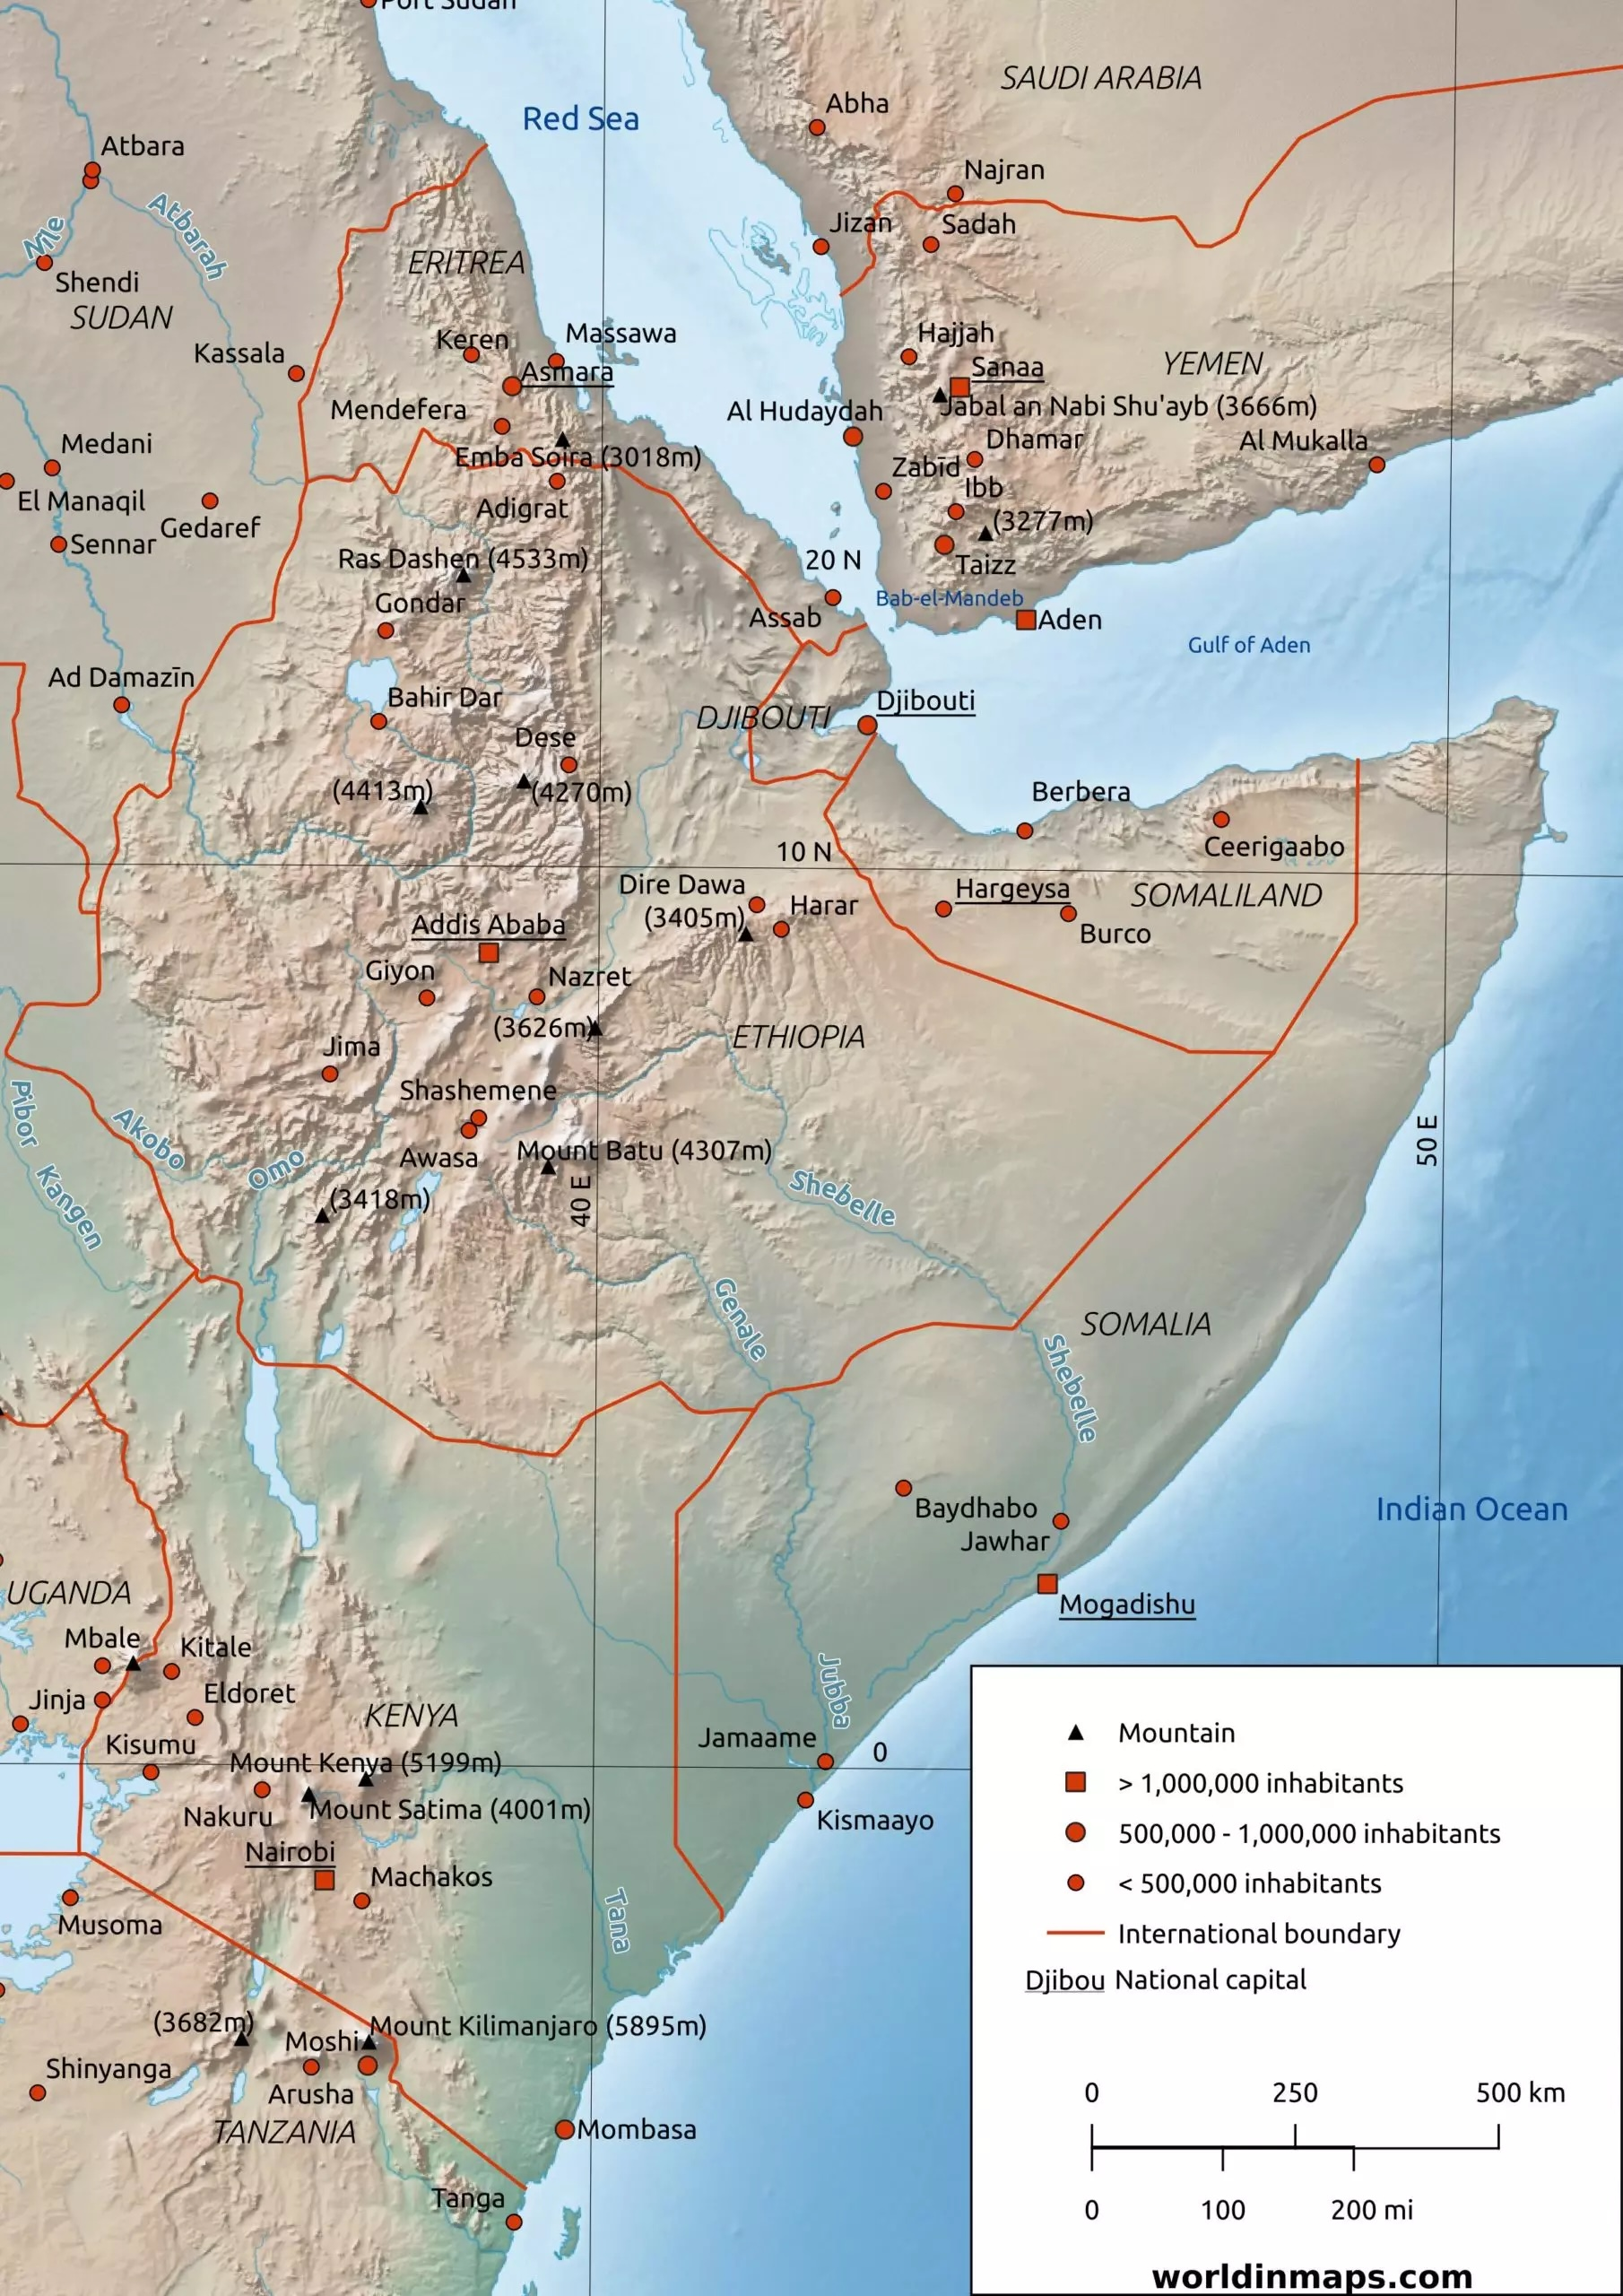
\includegraphics[width=0.6\textwidth]{../figures/static/horn-of-africa-map-scaled.jpeg}
    \caption{Map of the Horn of Africa \citep{WorldInMaps2024}}
    \label{fig:horn-of-africa}
\end{figure}

The region is also geographically diverse, with a range of topographical features that influence local weather patterns (Figure \ref{fig:horn-of-africa}). From the west, the Sahel fades into the Ethiopian Highlands and later the East African Rift Valley, which is characterised by high topographic relief and complex orography. These highlands then transition into the low-lying coastal plains of Somalia. Unlike most other countries at this latitude, most of Somalia is arid or semi-arid, with the exception of its border region with Kenya \citep{Beck2023}. This contrast in geography is reflected in storm development and rainfall patterns. The mountains of Ethiopia dominate local convective processes while the low-lying areas on the south-eastern coast of the region are not nearly as conducive to \acrshort{mcs} development \citep{Negash2024,Camberlin2024}. Thus, the coast is much more susceptible to storm patterns over the Indian Ocean and the Gulf of Aden \citep{Camberlin2024}. The combination of land surface skin temperature and soil moisture also impact the storm development and intensification. Notably, multiple studies over distinct regions have demonstrated that strong soil moisture gradients can intensify convection \citep{Barton2021,Klein2020,Taylor2017}. These processes are likewise relevant to the Horn of Africa, especially in transitional climates bridging arid and humid zones.

The primary challenge in rainfall prediction is that \acrfull{nwp} models have historically not operated at high enough resolutions to resolve convective processes and instead use sub-grid parametrisation schemes to more accurately replicate storm behaviour \citep{Stevens2019,Yano2018}. Newer kilometre-scale models are showing promise in more faithfully representing these processes, but large discrepancies still exist between model outputs and observed phenomena \citep{Feng2025,Yano2018}. For example, these models tend to underestimate \acrshort{mcs} precipitation totals while overestimating the intensity of precipitation \citep{Feng2025,Stevens2019}. Further complicating the modelling landscape is the mid-latitude bias of many \acrshort{nwp} models, which tend to perform worse in the tropics and subtropics at shorter lead times \citep{Keane2025}. 

In addition, the entire continent of Africa is considerably under-represented in high-quality meteorological data and many national meteorological services lack critical resources to more effectively monitor and predict \acrshortpl{mcs} \citep{Dinku2019,Kinyondo2018,Meque2021}. This discrepancy also has downstream effects on global meteorology, as reanalysis datasets and digital twin systems rely heavily on data assimilation of observations and regional models for calibration \citep{Linsenmeier2023,Valmassoi2023}. 

Although increased investment and study are undoubtedly necessary, these challenges present an opportunity for innovative methods in the immediate term to make use of existing data to better understand \acrshort{mcs} behaviour. Targeted insights into the factors which contribute to storm intensification and propagation could help inform the design of new observational networks, improve sub-grid parametrisation schemes, and ultimately lead to better forecasts. This is especially imperative in a region like Africa where computational resources are limited, and the need for short-range forecast accuracy is critical. This thesis intends to address said challenges by presenting a reusable, \acrfull{xai}-based framework to identify and analyse important factors for \acrshort{mcs} intensification and propagation.

\section{Explainable Artificial Intelligence for Convective Systems}

The field of meteorology has been no exception to the increasing popularity of data-driven research methods. Ample amounts of manual observations spanning nearly centuries, petabytes of satellite imagery, the output of numerical models and reanalysis datasets like the \acrfull{era5} and \acrfull{merra2} constitute a rich repository of training and validation data \citep{Bracco2024,Waqas2024,Zhang2025}. Given the complexity of atmospheric processes, there are numerous opportunities at varying scales to improve our understanding and prediction of weather and climate phenomena. On the smaller scale, \acrfull{ml} has been used for tasks such as downscaling, parametrisation, and nowcasting, where the goal is to improve the resolution and accuracy of existing numerical forecasts \citep{Blunn2024,Zhang2023}. On the larger scale, an especially popular approach known as \acrfull{piml} incorporates constraints directly into the training process to penalise the models for not adhering to the laws of physics \citep{Pathak2022,Luo2025,Zhang2023}.

In spite of the rapid emergence and success of these methods, the fundamental challenge of trustworthiness remains. This is particularly important in domains like meteorology where understanding the rationale behind predictions is crucial \citep{BarredoArrieta2019,Zhang2025}. As a result, there is a growing interest in developing methods for explainable and interpretable \acrshort{ml}, known as \acrfull{xai}, to provide insights into the decision-making processes of these models. There are many such methods including models which are inherently interpretable by design, like linear regression, as well as post-hoc explanation methods, for instance \acrfull{shap}, which can be applied to any model after training \citep{BarredoArrieta2019,Molnar2025}. Unsurprisingly, \acrshort{xai} deployment has also increased across different domains in meteorology, including weather prediction, climate modelling, and extreme event analysis \citep{Mamalakis2022,Yang2024}. More relevant for this thesis, \acrshort{xai} has been employed specifically for understanding convective systems. \cite{Bassine2025} and \cite{Zhang2019} use interpretable models to predict rainfall extremes in Africa and \acrshortpl{mcs} transition into tropical cyclones, respectively. \cite{Zhuo2021} used both \acrshort{piml} and the post-hoc explanation methods to estimate tropical cyclone intensity and size. While these studies span diverse meteorological applications, they underscore the growing potential of \acrshort{xai} for understanding and forecasting convective systems in particular.

The main inspiration for the methodology of this thesis comes from \cite{Hunt2024}'s investigation of interpretable gradient-boosted decision-trees for uncovering dynamical relationships governing \gls{indianmonsoon} \acrfullpl{lps}. They first utilised a tracking algorithm to assemble a database of \acrshort{lps} storm tracks from \acrshort{era5} data. Using the storm centroids along each track, they extracted a set of meteorological and geographic features from the surrounding \acrshort{era5} data. These features were then used to train gradient-boosted decision tree models to predict specific storm characteristics, like mean precipitation or peak vorticity. The model was then interpreted using \acrshort{shap} values to not only identify the most important features, but also reveal how feature importance changes relative to geography. Within the results, the authors found that processes affecting intensification differ from those affecting peak intensity and also confirmed existing research that mid-level winds are relevant for predicting storm speed and direction. This methodology is particularly compelling as it offers a framework that could be adapted for other regions and storm types with the only pre-requisite being high-quality storm track data.

However, there are also many additional paths for exploration, especially leveraging the explanatory power of \acrshort{shap} values. For example, \cite{Hunt2024} primarily focus on the model's ability to capture the relationships between features and storm characteristics, but do not explore the model's ability to predict storm tracks or propagation. While interpretable \acrshort{ml} techniques pale in comparison to traditional \acrshort{nwp} models, their insights may be able to aid with sub-grid parametrisation or facilitate the planning of new observational networks in data-scarce and computationally limited regions like Africa. Furthermore, while \cite{Hunt2024} do take great care to justify the inclusion of each feature and remove those that are highly correlated, they do not explore the possibility of direct comparison between models trained with different feature sets. This could be useful in disentangling the relative importance of meteorological and geographical features, which may often work in concert or direct opposition, such as wind angle and orography. Thus, this thesis aims to build upon their work by exploring these additional avenues and further investigating the potential of \acrshort{xai} techniques for understanding and predicting storm behaviour.

\section{Research Objectives}

The primary objective of this research is to investigate the factors which contribute to the intensification and propagation of East African \acrshortpl{mcs} through the usage of an interpretable machine learning model and subsequent application of \acrshort{xai} techniques. The methodology will largely follow the framework established by \cite{Hunt2024}, with adaptations made for the specific context of East African storms. A necessary pre-requisite for achieving this objective is the creation of a dataset that captures relevant meteorological features along the storm track. This will involve the integration of the East African \acrshort{mcs} database from \cite{Hill2023} with \acrshort{era5} reanalysis data. Next, multiple gradient-boosted decision tree models will be trained to predict various features of storm intensification and propagation using the aforementioned dataset and the \acrfull{xgb} Python library. The choice to use this modelling framework is motivated by its balance between predictive capacity and interpretability, as well as its ability to handle tabular data effectively. The models will be optimised using hyperparameter tuning and their performance compared between similar experiments with different feature sets to assess the impact of feature selection. Finally, \acrshort{xai} techniques, particularly \acrshort{shap}, will be employed to interpret the models' predictions and identify the key factors influencing storm behaviour.

\section{Report Structure}

The main body of this report is organised into four chapters with accompanying appendices which contain supplementary material including the full codebase and additional figures. The current chapter, Chapter~\ref{ch:intro}, provides an overview of the research context, objectives, and structure of the report. This includes relevant information on \acrshortpl{mcs} in East Africa, data-driven scientific discovery, \acrfull{xai}, and brief review of current applications of \acrshort{xai} for convective systems. Chapter~\ref{ch:method} will detail all aspects of the research methodology, detailing the East African \acrshort{mcs} database and \acrshort{era5} reanalysis, data processing, feature selection, model training, and the main \acrshort{xai} technique utilised, \acrshort{shap}. Chapter~\ref{ch:results} will present the experimental design and subsequent results. This will entail a comparison of the model performance on different feature sets and an analysis of feature importance using \acrshort{shap} values. This analysis will detail overall feature importance across models and experiments, but also further investigate how it varies over geography and time. Chapter~\ref{ch:results} will also explore the implications and limitations of the findings. Chapter~\ref{ch:con} concludes the report by summarising the key contributions and potential avenues for future research.
    \chapter{Background and Literature Review}
\label{ch:background}

% A literature review chapter can be organized in a few sections with appropriate titles. A literature review chapter might  contain the following:
% \begin{enumerate}
%     \item A review of the state-of-the-art (include theories and solutions) of the field of research.
%     \item A description of the project in the context of existing literature and products/systems.
%     \item An analysis of how the review is relevant to the intended application/system/problem.
%     \item A critique of existing work compared with the intended work.
% \end{enumerate}
% Note that your literature review should demonstrate the significance of the project.
% https://guides.library.bloomu.edu/litreview

% \section{State-of-the-art}

% \section{Critique of the review}

% \section{Summary} 

\section{Mesoscale Convective Systems (MCSs)}

Due to significant size, duration, and impact, \acrfullpl{mcs} constitute a critical component of regional weather forecasting and climatology. Officially, \acrshortpl{mcs} are defined as complex of thunderstorms which becomes organised on a scale larger than any of the individual thunderstorms \citep{NOAANWS2025}. Consequently, these storm systems often last for several hours and cover areas of tens of thousands of square kilometres. In addition, they often produce severe weather phenomena, including flooding, strong winds, and hail \citep{Houze2014}. Unlike many \Gls{synopticscale} systems, \acrshortpl{mcs} are not usually associated with a well-defined center of circulation and instead are characterized by their multi-scale organization, typically incorporating a variety of convective cells and larger-scale features such as squall lines or mesoscale convective complexes \citep{NOAANWS2025,AMS2024}. These systems are prevalent throughout the world and thus are key to understanding regional climatology. For example, in the United States, \acrshortpl{mcs} are a primary driver of warm-season precipitation over the Great Plains \citep{Haberlie2019}. The Sahel region of Africa produces some of the strongest \acrshortpl{mcs} globally due to it being a climatic transition zone with strong seasonal cycles \citep{Zipser2006}.

\subsection{MCSs in the Horn of Africa}

While the Horn of Africa is a region with complex topography and large-scale climatic variability affecting the development of \acrshortpl{mcs}, it has been shown that the systems still contribute to over 60\% of extreme rainfall in Ethiopia and Somalia \citep{Hill2023}. From the west, the Sahel fades into the Ethiopian Highlands and later the East African Rift Valley, characterized by high topographic relief and complex orography. In the east, the Ethiopian Highlands transition into the low-lying coastal plains of Somalia. Unlike most other countries at this latitude, most of Somalia is arid or semi-arid, with the exception of its border region with Kenya \citep{Beck2023}. This contrast in geography is reflected in storm development and precipitation patterns. The mountains of Ethiopia dominate local convective processes \citep{Negash2024} while the low-lying areas on the southeastern coast of the region are not nearly as conducive to \acrshort{mcs} development and thus are much more susceptible to storm patterns over the Indian Ocean and the Gulf of Aden \citep{Camberlin2024}. The combination of land surface temperature and soil moisture also impact the storm development and intensification. Notably, studies in the Sahel have demonstrated that dry soils downstream of moisture anomalies can intensify convection by strengthening low-to-mid-level wind shear \citep{Klein2020,Taylor2017}. These processes are similarly relevant to the Horn of Africa, especially in transitional climates bridging arid and humid zones.

Large-scale \glspl{teleconnection} also play a major role in governing \acrshort{mcs} activity in this region. The \acrfull{mjo} is a dominant intraseasonal factor which modulates rainfall in the tropics and in East Africa, its active phases coincide with increased convection and extreme rainfall events \citep{Pohl2006,Ochieng2023}. Quite uniquely for the tropics, the \acrfull{itcz} passes over the region twice per year leading to two distinct rainy seasons, one short and one long \citep{Palmer2023,Tefera2025}. The \acrfull{enso} and the \acrfull{iod} have also been shown to modulate rainfall patterns in the region, with coupled regional climate models able to reproduce these patterns at various timescales \citep{Vashisht2021,Dubache2019,Endris2019}.


    \chapter{Data}
\label{ch:data}

\begin{itemize}
    \item \textbf{Database of East African Mesoscale Convective Systems (MCSs)}
    \begin{itemize}
        \item File: \texttt{East\_Africa\_tracked\_MCSs\_2014\_2019\_longer\_than\_3\_hours.csv}
        \item Contains 27,982 storms longer than 3 hours, with all storm centroids along the track within (3--15N, 34--52E)
    \end{itemize}
    \item \textbf{ERA5 Data}
    \begin{itemize}
        \item ERA5 data for 31--53E, 2--16N region for 2014--2019, totaling 27 GB
        \item The ERA5 area is slightly wider by a few grid points to account for edge cases in the database and for calculating gradients
    \end{itemize}
\end{itemize}
    \chapter{Methodology}
\label{ch:method}

This section details the methodology employed in this research. The approach is structured into several key components: data collection and processing, the modelling approach, and model explainability.

\section{Data}

\subsection{Database of East African Mesoscale Convective Systems (MCSs)}

In their paper, \cite{Hill2023} used a variant of the "simple-track" object tracking algorithm to identify and track \acrshortpl{mcs} over East Africa from infrared satellite imagery over 2014 to 2019 \citep{Stein2020}. The tracking algorithm identifies contiguous areas of cloud top brightness temperature (BT)\todo{acronym, especially to help table below?} below a threshold of \SI{233}{\kelvin}. The algorithm then tracks these areas over time based on their spatial overlap in consecutive images. The resulting database contains detailed information on the location, size, intensity, and duration of each \acrshort{mcs}, as well as precipitation amounts derived from Global Precipitation Measurement (GPM) satellite imagery.

From this comprehensive storm database, a subset of approximately 30,000 was selected for analysis. Two criteria were used to filter for storms relevant to this study: 1) storms must be longer than 3 hours, and 2) all storm centroids must be located within the geographical bounds of (\degN{3} - \degN{15}, \degE{34} - \degE{52}). The 3-hour threshold was chosen because storms of this duration account for 92\% of \acrshort{mcs} precipitation \citep{Hill2023}.

\subsection{ERA5 Data}

\acrfull{era5} is a reanalysis dataset produced by the \acrfull{ecmwf} which includes atmospheric, land, and oceanic climate variables from 1950 onwards \citep{Hersbach2020}. For this thesis, hourly data separated into yearly files was downloaded from the Copernicus Climate Change Service (C3S) Climate Data Store (CDS). The region for the data download was chosen to be slightly larger than the storm database region, covering (\degN{2} - \degN{16}, \degE{31} - \degE{53}). This buffer ensures that all storms are fully captured and to facilitate the calculation of gradients. The data was downloaded at a spatial resolution of \SI{0.25}{\degree} and includes the following meteorological variables relevant to storm development and propagation.

\begin{table}[ht]
    \centering
    \caption{ERA5 Data File Patterns, Descriptions, and Units}
    \label{tab:era5-file-patterns}
    \begin{tabular}{p{0.25\linewidth} p{0.45\linewidth} p{0.2\linewidth}}
        \toprule
        File Pattern & Description & Units/Notes \\
        \midrule
        \texttt{cape\_0\_YEAR.nc} & Convective available potential energy & \unit{\joule\per\kilogram} \\
        \texttt{olr\_toa\_YEAR.nc} & Top-of-atmosphere outgoing longwave flux (proxy for convection/clouds) & \unit{\watt\per\meter\squared} \\
        \texttt{prcp\_tot\_YEAR.nc} & Thickness of rainfall amount (hourly accumulations) & \unit{\meter} \\
        \texttt{rhum\_PRESSURE\_YEAR.nc} & Relative humidity at 500, 750 and 900 \unit{\hecto\pascal} & \unit{\percent} (used for theta e calculations) \\
        \texttt{shum\_PRESSURE\_YEAR.nc} & Specific humidity at 200, 500, 850 \unit{\hecto\pascal} & \unit{\kilogram\per\kilogram} \\
        \texttt{skt\_sfc\_YEAR.nc} & Surface temperature on land & \unit{\kelvin} \\
        \texttt{sst\_sfc\_YEAR.nc} & Sea surface temperature & \unit{\kelvin} \\
        \texttt{swvl1\_d1\_YEAR.nc} & Volumetric soil water layer 1 & \unit{\meter\cubed\per\meter\cubed} \\
        \texttt{swvl2\_d2\_YEAR.nc} & Volumetric soil water layer 2 & \unit{\meter\cubed\per\meter\cubed} \\
        \texttt{ta\_PRESSURE\_YEAR.nc} & Air temperature at 500, 750 and 900 \unit{\hecto\pascal} & \unit{\kelvin} (used for theta e calculations) \\
        \texttt{tcwv\_tot\_YEAR.nc} & Thickness of atmosphere mass content of water vapour & \unit{\kilogram\per\meter\squared} (total column water vapour) \\
        \texttt{thetae\_PRESSURE\_YEAR.nc} & Equivalent potential temperature at 500, 750 and 900 \unit{\hecto\pascal} & \unit{\kelvin} (dew point, LCL temperature, theta e via MetPy) \\
        \texttt{uwnd\_PRESSURE\_YEAR.nc} & Zonal wind at 200, 500 and 850 \unit{\hecto\pascal} & \unit{\meter\per\second} \\
        \texttt{vwnd\_PRESSURE\_YEAR.nc} & Meridional wind at 200, 500 and 850 \unit{\hecto\pascal} & \unit{\meter\per\second} \\
        \bottomrule
    \end{tabular}
\end{table}


\subsection{Feature Engineering and Selection}

Table \ref{tab:features} describes the X features used for this thesis and their respective units. These features were derived from the original storm database and \acrshort{era5} data through a series of processing steps. The features can be broadly categorised into three groups: storm-specific features, meteorological features, and geographical features. Features with the \texttt{mean\_} prefix are calculated over a 400 km radius square-area from the \acrshort{mcs} centre and are instantaneous unless otherwise specified. Features with the \texttt{domain\_mean\_} prefix are calculated over the entire domain of the \acrshort{era5} and are also instantaneous unless otherwise specified. The \SI{400}{\km} radius was chosen to align with the original study by \cite{Hunt2024} and to capture the mesoscale environment surrounding each storm. The features without these prefixes are either directly sourced from the storm database or are derived from the \acrshort{era5} data at the grid points corresponding to the storm centroids.

{\small
\begin{longtable}{>{\raggedright\arraybackslash}p{0.25\linewidth} p{0.50\linewidth} >{\raggedright\arraybackslash}p{0.15\linewidth}}
    \caption{Features Used in the Study. Long feature names are wrapped for readability.} \\
    \label{tab:features} \\
    \toprule
    \textbf{Feature name} & \textbf{Description} & \textbf{Units} \\
    \midrule
    \endfirsthead

    \multicolumn{3}{c}%
    {{\bfseries \tablename\ \thetable{} -- continued from previous page}} \\
    \toprule
    \textbf{Feature name} & \textbf{Description} & \textbf{Units} \\
    \midrule
    \endhead

    \midrule \multicolumn{3}{r}{{Continued on next page}} \\
    \endfoot

    \bottomrule
    \endlastfoot

    \texttt{date\_angle} & Angle representation of current date within year & \unit{\degree} \\
    \texttt{eat\_hours} & Time step hour of day & \href{https://www.timeanddate.com/time/zones/eat}{Eastern Africa Time} (UTC+3) \\
    \texttt{storm\_total\_duration} & Total duration of \acrshort{mcs} & \unit{\hour} \\
    \texttt{lon} & Longitude of \acrshort{mcs} centre & \unit{\degree}E \\
    \texttt{lat} & Latitude of \acrshort{mcs} centre & \unit{\degree}N \\
    \texttt{orography\_height} & Elevation of land surface at \acrshort{mcs} centre & \unit{\meter} \\
    \texttt{anor} & Angle of sub-gridscale orography at \acrshort{mcs} centre & radians from E \\
    \texttt{upslope\_bearing} & Compass bearing of upslope direction at \acrshort{mcs} centre & \unit{\degree} from  N \\
    \texttt{slope\_angle} & Angle of slope at \acrshort{mcs} centre & \unit{\degree} \\
    \texttt{over\_land} & Flag for \acrshort{mcs} centre (True if \acrshort{mcs} centre is over land, else False) & \texttt{boolean} \\
    \texttt{acc\_land\_time} & Accumulated time where \texttt{over\_land}=True & \unit{\hour} \\
    \texttt{storm\_total\_land\_time} & Final value of \texttt{acc\_land\_time} for \acrshort{mcs} & \unit{\hour} \\
    \texttt{mean\_land\_frac} & Fraction of area within 400 km that is over land & ratio ($[0,1]$) \\
    \texttt{zonal\_speed} & $x$-component of \acrshort{mcs} centre propagation vector & \unit{\km\per\hour} \\
    \texttt{meridional\_speed} & $y$-component of \acrshort{mcs} centre propagation vector & \unit{\km\per\hour} \\
    \texttt{area} & Area of the \acrshort{mcs} & \unit{\km\squared} \\
    \texttt{storm\_max\_area} & Max value of \texttt{area} for \acrshort{mcs} & \unit{\km\squared} \\
    \texttt{bearing\_from\_prev} & Compass bearing from previous observation & \unit{\degree} from  N \\
    \texttt{bearing\_to\_next} & Compass bearing to next observation & \unit{\degree} from  N \\
    \texttt{distance\_from\_prev} & Distance traversed from previous observation & \unit{\km} \\
    \texttt{distance\_to\_next} & Distance to next observation & \unit{\km} \\
    \texttt{distance\_traversed} & Cumulative sum of \texttt{distance\_from\_prev} & \unit{\km} \\
    \texttt{storm\_bearing} & Compass bearing from first to last \acrshort{mcs} centre & \unit{\degree} from  N \\
    \texttt{storm\_distance \_traversed} & Total cumulative distance traversed by \acrshort{mcs} centre & \unit{\km} \\
    \texttt{storm\_straight \_line\_distance} & Distance from first to last \acrshort{mcs} centre & \unit{\km} \\
    \texttt{mean\_skt} & Surface temperature & \unit{\kelvin} \\
    \texttt{mean\_land\_skt} & Land surface temperature (\acrshort{nan} if entire area is ocean) & \unit{\kelvin} \\
    \texttt{mean\_sst} & Sea surface temperature (\acrshort{nan} if entire area is land) & \unit{\kelvin} \\
    \texttt{mean\_swvl1} & Volumetric soil moisture in the top layer ($<$7 cm; NaN over ocean) & \unit{\meter\cubed\per\meter\cubed} \\
    \texttt{mean\_swvl2} & Volumetric soil moisture in the second layer (7--28 cm; NaN over ocean) & \unit{\meter\cubed\per\meter\cubed} \\
    \texttt{mean\_u850} & \SI{850}{\hecto\pascal} zonal wind & \unit{\meter\per\second} \\
    \texttt{mean\_u500} & \SI{500}{\hecto\pascal} zonal wind & \unit{\meter\per\second} \\
    \texttt{mean\_u200} & \SI{200}{\hecto\pascal} zonal wind & \unit{\meter\per\second} \\
    \texttt{mean\_v850} & \SI{850}{\hecto\pascal} meridional wind & \unit{\meter\per\second} \\
    \texttt{mean\_v500} & \SI{500}{\hecto\pascal} meridional wind & \unit{\meter\per\second} \\
    \texttt{mean\_v200} & \SI{200}{\hecto\pascal} meridional wind & \unit{\meter\per\second} \\
    \texttt{domain\_mean\_u500} & Mean \SI{500}{\hecto\pascal} zonal wind over the entire domain of ERA5 data & \unit{\meter\per\second} \\
    \texttt{mean\_u\_shear\_850\_500} & Shear of zonal wind from \SI{850}{\hecto\pascal} to \SI{500}{\hecto\pascal} & \unit{\meter\per\second} \\
    \texttt{mean\_v\_shear\_850\_500} & Shear of meridional wind from \SI{850}{\hecto\pascal} to \SI{500}{\hecto\pascal} & \unit{\meter\per\second} \\
    \texttt{mean\_u\_shear\_850\_200} & Shear of zonal wind from \SI{850}{\hecto\pascal} to \SI{200}{\hecto\pascal} & \unit{\meter\per\second} \\
    \texttt{mean\_v\_shear\_850\_200} & Shear of meridional wind from \SI{850}{\hecto\pascal} to \SI{200}{\hecto\pascal} & \unit{\meter\per\second} \\
    \texttt{wind\_direction\_850} & Compass bearing from which the \SI{850}{\hecto\pascal} wind vector at \acrshort{mcs} centre originates & \unit{\degree} from  N \\
    \texttt{wind\_angle\_upslope} & Angle of \texttt{wind\_direction\_850} relative to \texttt{upslope\_bearing} (wind is going upslope: \ang{0}, downslope: \ang{180}, cross-slope: \ang{90}, \ang{270}) & \unit{\degree} from \texttt{upslope\_bearing} \\
    \texttt{mean\_tcwv} & Total column water vapour (TCWV) & \unit{\kilogram\per\meter\squared} \\
    \texttt{domain\_mean\_tcwv} & Mean TCWV over the entire domain of ERA5 data & \unit{\kilogram\per\meter\squared} \\
    \texttt{mean\_q\_850} & \SI{850}{\hecto\pascal} specific humidity & \unit{\kilogram\per\kilogram} \\
    \texttt{mean\_q\_500} & \SI{500}{\hecto\pascal} specific humidity & \unit{\kilogram\per\kilogram} \\
    \texttt{mean\_q\_200} & \SI{200}{\hecto\pascal} specific humidity & \unit{\kilogram\per\kilogram} \\
    \texttt{mean\_cape} & Convective available potential energy (CAPE) & \unit{\joule\per\kilogram} \\
    \texttt{domain\_mean\_cape} & Mean CAPE over the entire domain of ERA5 data & \unit{\joule\per\kilogram} \\
    \texttt{olr\_90} & 90th percentile of negative outgoing longwave radiation (OLR) within 400 km & \unit{\watt\per\square\meter} \\
    \texttt{olr\_75} & 75th percentile of negative OLR within 400 km & \unit{\watt\per\square\meter} \\
    \texttt{olr\_50} & 50th percentile of negative OLR within 400 km & \unit{\watt\per\square\meter} \\
    \texttt{mean\_prcp\_400} & Precipitation over the next 6 hr & \unit{\milli\meter} \\
    \texttt{min\_bt} & Minimum cloudtop brightness within \acrshort{mcs} area & \unit{\kelvin} \\
    \texttt{dmin\_bt\_dt} & Rate of change of \texttt{min\_bt} & \unit{\kelvin\per\hour} \\
    \texttt{mean\_bt} & Mean cloudtop brightness within \acrshort{mcs} area & \unit{\kelvin} \\
    \texttt{dmean\_bt\_dt} & Rate of change of \texttt{mean\_bt} & \unit{\kelvin\per\hour} \\
    \texttt{storm\_min\_bt} & Minimum value of \texttt{min\_bt} reached for \acrshort{mcs} & \unit{\kelvin} \\
    \texttt{storm\_min\_bt\_reached} & False if \texttt{storm\_min\_bt} has not been reached yet, else True & \texttt{boolean} \\
    \texttt{mjo\_phase} & Phase of Madden--Julian oscillation (MJO) & $[1, 8] \cap \mathbb{Z}$ \\
    \texttt{mjo\_amplitude} & Amplitude of MJO & - \\
\end{longtable}
}

The following highly correlated features were identified and removed to prevent redundancy and reduce the risk of multicollinearity, which can negatively impact model interpretability and performance.  A full correlation heatmap is available in Appendix \insertref{app:correlation-heatmap}.
\begin{itemize}
    \item \texttt{mean\_swvl1} and \texttt{mean\_swvl2} have a Pearson correlation coefficient of 0.94 and thus \texttt{mean\_swvl2} was removed.
    \item \texttt{olr\_90}, \texttt{olr\_75}, \texttt{olr\_50} were all correlated with coefficients above 0.8, so only \texttt{olr\_90} was retained.
\end{itemize}
Additionally, measures were implemented to prevent data leakage, including the careful exclusion of features that are directly related to the target variable or contain information from future time steps that would not be available at prediction time. These steps help ensure that the model learns meaningful relationships from the data and that its predictive performance is not artificially inflated by access to information that would not be present in a real-world forecasting scenario.

\section{Modelling Approach}

The following section describes the \acrshort{ml} approach taken to predict storm intensification and propagation. As all predictands are continuous variables and the input features can be directly associated with the target storm characteristics, this \acrshort{ml} task is classified as supervised regression as opposed to unsupervised learning, where the target variables are not known, or classification, where the goal is to predict discrete labels.

\subsection{XGBoost}

In this thesis, \acrfull{xgb} is the modelling framework employed for this supervised regression task. In part, the decision to use \acrshort{xgb} corresponds with faithfully reproducing the methodology of \cite{Hunt2024}. However, their choice is justified by the advantages that the approach presents. \acrshort{xgb} is a decision-tree based model leveraging an efficient and scalable implementation of gradient boosting \citep{Chen2016}. Gradient boosting, an extension of \gls{ensemblelearning}, iteratively trains weak learners, in this case decision trees, on the residual errors of the previous learners. This process allows the model to focus on the most challenging examples to improve overall performance while also preventing overfitting, especially when compared to one, highly complex decision tree model \citep{Friedman2001}. Yet, since the model retains the underlying structure of decision trees, it remains directly interpretable through techniques like feature importance. Generally, feature importance is a global model-agnostic \acrshort{xai} method that quantifies the contribution of each feature to the model's predictions by measuring the change in the model's performance when the feature is permuted \citep{Musolf2022}. In decision-tree based models, the nature of the trees themselves can be exploited to more efficiently calculate importance. Typically, this is based on metrics like the frequency with which a feature is used for splitting, the average gain in accuracy from splits involving that feature, or the total reduction in impurity attributed to that feature across all trees in the ensemble \citep{Louppe2013}. Although not used in this thesis, the inherent interpretability of \acrshort{xgb} through feature importance analysis aligns with the goals of this research.

\subsection{Hyperparameter Tuning}

\acrshort{xgb} provides a myriad of hyperparameters that can be adjusted to optimise model performance. These include parameters controlling the learning rate, tree depth, number of trees, and regularisation terms, among others. The choice of hyperparameters can significantly impact the model's ability to generalise to unseen data. Therefore, a systematic approach to hyperparameter tuning is essential. 

In this thesis, hyperparameter tuning is conducted using \acrfull{wandb}, a popular web-based tool for tracking and visualising \acrshort{ml} experiments \citep{Biewald2020}. Specifically, Bayesian optimisation is employed to efficiently explore the hyperparameter space and identify optimal configurations. Bayesian optimisation is particularly well-suited for this task as it builds a probabilistic model of the cost function and uses it to select the most promising hyperparameters to evaluate next \citep{Mockus1994,Shahriari2016}\todo{better desc/wording}. This approach balances exploration and exploitation, allowing for a more efficient search compared to grid or random search methods. 

For regression tasks, many metrics can be used to evaluate model performance. In this thesis, \acrfull{rmse} is used because, by square rooting the mean of the squared errors, it provides a measure of error in the same units as the original predictions and is therefore more interpretable. Thus, Bayesian optimisation is set to minimise the validation \acrshort{rmse} during hyperparameter tuning. By default, \acrshort{wandb} sweeps will continue until manually stopped unless a maximum trial count is provided. For this thesis, a maximum trial count of 20 is used. \todo{this value might change}

Additionally, cross-validation is utilised during training on each trial to ensure that the model's performance is robust and not overly dependent on a specific subset of the data. Specifically, the dataset is first split into a training set and a test set to ensure that some data remains completely unseen throughout the training process. Then, within the training set, k-fold cross-validation is applied, where the dataset is divided into k subsets and the model is trained and validated k times, each time using a different subset as the validation set and the remaining subsets for training. Once all folds are complete, the best performing model is chosen as the result of the trial. This method provides a more reliable estimate of model performance on the given hyperparameters \citep{Lopez2023,Singh2021}\todo{better desc/wording}.

The specific hyperparameters tuned and the corresponding values or distributions used for the sweep are included in Table \ref{tab:wandb-sweep-config}. The remaining hyperparameters were kept at their default values as defined in the \acrshort{xgb} Python implementation \insertref{need a link to xgb docs here similar to Hunt2024?}.

\begin{table}[!ht]
    \centering
    \caption{\acrshort{wandb} Sweep Configuration for \acrshort{xgb} Hyperparameter Tuning. The names in this table refer to the hyperparameter names for the Scikit-Learn wrapper interface for \acrshort{xgb}. A full description of each hyperparameter can be found in the \href{https://xgboost.readthedocs.io/en/stable/python/python_api.html\#module-xgboost.sklearn}{XGBoost documentation}.}
    \label{tab:wandb-sweep-config}
    \begin{tabular}{llr}     
        \toprule
        \textbf{Hyperparameter} & \textbf{Values / Distribution} \\ 
        \midrule
        Gamma ($\gamma$) & Uniform[0, 5] \\
        Regularisation Alpha ($\alpha$) & Uniform[0, 5] \\
        Regularisation Lambda ($\lambda$) & Uniform[0, 5] \\
        Column Subsample by Tree & Uniform[0, 1.0] \\
        Learning Rate & Uniform[0, 1.0] \\
        Max Depth & \{3, 6, 9, 12\} \\
        Number of Estimators & \{60, 120, 180\} \\
        \bottomrule
    \end{tabular}
\end{table}

Once the sweeps are complete, the best models from each sweep are evaluated on the held-out test set to provide an unbiased estimate of their performance. The test \acrshort{rmse} values are first compared with the standard deviation of the target variable in the test set to assess whether the model has successfully captured novel relationships beyond just the underlying distribution of the target. They are then compared across different models and feature sets to assess relative performance. Furthermore, test \acrshort{rmse} over the dataset region and time period is analysed to identify any spatial or temporal patterns in model performance. \todo{if no time, this is for future work section}

\section{Model Explainability}
\todo{copied from background; will need to be adapted}

\acrfull{xai} is an emerging field focused on developing methods and techniques to make the decision-making processes of \acrshort{ml} solutions more transparent and easier to understand. Approaches in this field take a variety of forms, including inherently interpretable models and post-hoc explanation methods. A summary of \acrshort{xai} taxonomy is given in Figure \ref{fig:xai-taxonomy}.

\begin{figure}[ht]
    \centering
    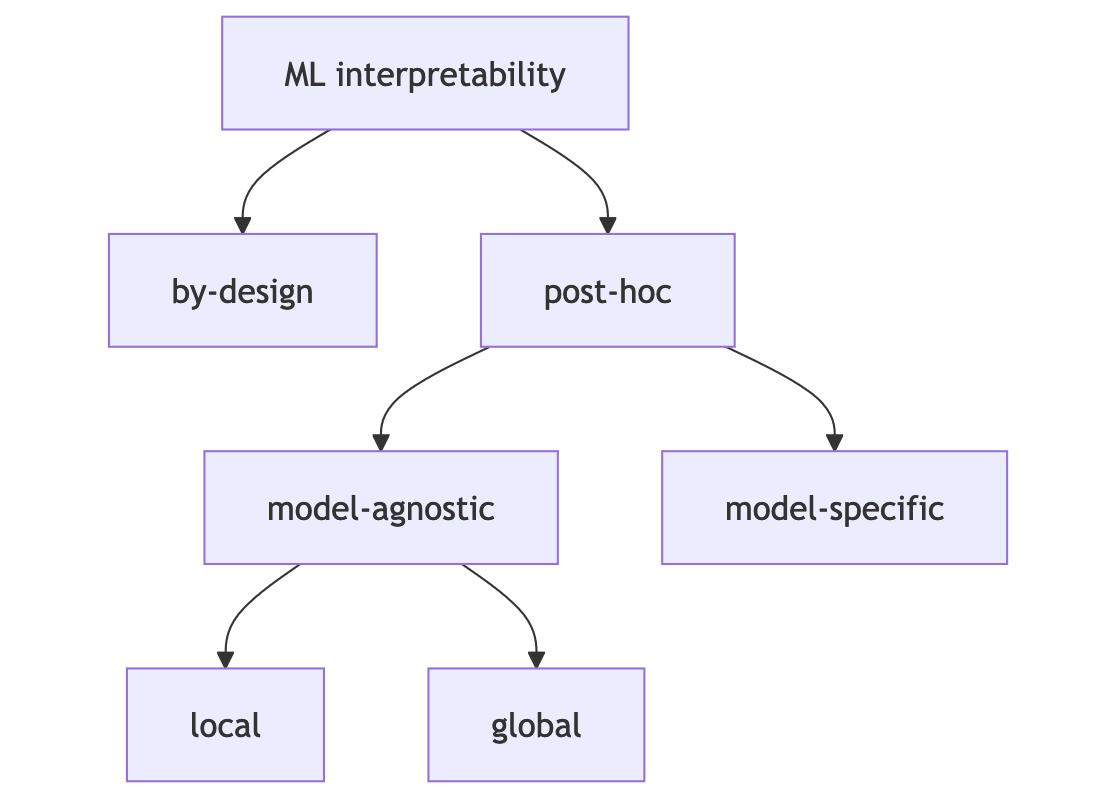
\includegraphics[width=0.8\textwidth]{../figures/static/xai-taxonomy.jpg}
    \caption{\acrshort{xai} Taxonomy \citep{Molnar2025}}
    \label{fig:xai-taxonomy}
\end{figure}

Inherently interpretable models are designed to be transparent by construction, often using simpler architectures or feature-based approaches that allow for direct interpretation of the relationship between inputs and outputs. Examples include linear regression, decision trees, and rule-based systems. A clear disadvantage is that these simpler models may sacrifice some predictive performance compared to more complex ones like \acrfull{dnn}. \acrshort{piml} could also be considered a part of this landscape, as it aims to integrate existing physical knowledge into architectures and training processes to enhance forecast accuracy and credibility \citep{Luo2025,Pathak2022}. Post-hoc explanation methods, on the other hand, are applied to models after training to partially interpret their behaviour. Model-specific post-hoc methods leverage the learned structure of the model. Feature importance, as mentioned above, serves as a illustrative example, where the decision-tree model structure is integrated directly into the explanation algorithm. Notably for this research, model-agnostic methods are predominantly designed to make no assumptions about a model's underlying architecture. These methods can then be broadly categorised into local and global explanations. Local explanations focus on providing insights into model behaviour around a given input. In contrast, global explanations aim to provide an overall understanding of the model's behaviour for any input. For local explanations, counterfactual analysis has gained traction, especially for classification tasks, where the model's local decision boundary can be more interactively explored through slight perturbations of the a given input \citep{Mothilal2019}. \acrfull{shap} is both applicable for local and global explanations and will be used extensively throughout this research. As such, a brief overview of the approach follows.

\subsection{Shapley Additive Explanations}

After its popularisation via \cite{Lundberg2017} and the accompanying \texttt{shap} \texttt{python} library, \acrfull{shap} has emerged as one of the most prominent frameworks for post-hoc explainability. This is achieved through the application of coalitional game theory where the algorithm approximates a fair distribution of "payout", in this case a fraction of the model's prediction, among the input features based on their individual contributions to the prediction \citep{Shapley1953}. Formally, the Shapley value for a feature is calculated via the average marginal contribution of that feature across all possible coalitions of features weighted by the probability of the coalition, where a coalition is a subset of features, and the marginal contribution of a feature to a coalition is the difference in the model's prediction when that feature is included versus when it is excluded. This process ensures that each feature's contribution is fairly evaluated by accounting for its interactions with other features. The result is a set of Shapley values for each feature and model output, which can then be used to interpret the model's predictions locally, by highlighting the most influential features for a single output, or globally, by aggregating the Shapley values across multiple predictions to identify overall feature importance.

In practice, this algorithm experiences a \gls{combinatorialexplosion} as features increase, thus, various approximations and optimisations have been developed to make it feasible for larger datasets. For example, \cite{Lundberg2017} present a kernel-based method which operates on the assumption that not all coalitions are equally important in quantifying a features marginal contribution. The application of Shapley values for explaining \acrshort{ml} models was first proposed by \cite{trumbelj2011}, but \cite{Lundberg2017} key contribution was the introduction of an additive feature attribution model, which allows for efficient approximation using a linear model. This approach assumes that the prediction can be expressed as a sum of the feature contributions, making it easier to interpret and visualise. The \texttt{shap} library implements both model-specific and agnostic methods using this framework and provides various tools for visualising Shapley values and their impact on individual predictions and overall model performance.

In this thesis, \acrshort{shap} is primarily used as a global explanation method. The goal is to identify the most important features driving model predictions across the entire dataset. This is achieved by calculating the mean absolute Shapley value for each feature across all predictions, which provides a measure of overall feature importance. The results are visualised using summary plots to simultaneously convey both the magnitude and direction of each feature's impact on the model's predictions. In addition, the spatial and temporal distribution of feature importance will be analysed to identify any regional or temporal patterns in the model's behaviour. Potential candidate features will be identified by correlating Shapley values with observation coordinates and timestamps. Top candidates will be analysed by mapping their Shapley values across the study region and time period. Such analyses are aimed to uncover which features are most dependent on location and time, potentially revealing underlying physical relationships captured by the model.

\section{Experimental Setup}

The experimental setup is designed to systematically evaluate the performance of the proposed models under different conditions and feature sets. The experiments are divided into two groups: storm aggregate characteristic prediction tasks and immediate characteristics at observation prediction tasks. Storm aggregate tasks involve predicting characteristics that summarise the entire lifecycle of a storm with the aim of understanding its overall behaviour and impact. In contrast, immediate characteristic tasks focus on predicting properties at each observation time step, such as the 6-hour mean precipitation or the rate of intensification. These tasks require a more granular understanding of the storm's evolution and are more applicable to real-time forecasting applications.

For all experiments, two models were trained on two different feature sets: all available features and only ERA5 meteorological features. This approach allows for a comparison of model performance when utilising a focused subset of variables. While it is likely that storm genesis location and orography over the track will play a major role, it is possible that those features could confound the effects of other environmental factors, like soil moisture or skin temperature. Thus, through this setup, we ensure that one model is exclusively learning from the meteorological conditions. If model performance differs significantly, this would imply that the geographic, topological, or temporal features contain unique information not captured by the meteorological features. Through a comparison of relative feature importance of the meteorological features, we can also gain insights into their interaction with the other features. In addition, for the storm aggregate prediction tasks, two additional models were trained using only the first observation of each storm, again comparing all features versus only ERA5 features. This aspect of the setup aims to evaluate the predictive power of initial storm observations.

The experiments conducted are summarised in Table \ref{tab:experimental-setup}.

{\small
\begin{longtable}{>{\raggedright\arraybackslash}p{0.27\linewidth} p{0.43\linewidth} >{\raggedright\arraybackslash}p{0.20\linewidth}}
    \caption{Experiments Summary. Long experiment names are wrapped for readability.} \\
    \label{tab:experimental-setup} \\
    \toprule
    \textbf{Experiment alias} & \textbf{Description} & \textbf{Predictand} \\
    \midrule
    \endfirsthead

    \multicolumn{3}{c}%
    {{\bfseries \tablename\ \thetable{} -- continued from previous page}} \\
    \toprule
    \textbf{Experiment alias} & \textbf{Description} & \textbf{Predictand} \\
    \midrule
    \endhead

    \midrule \multicolumn{3}{r}{{Continued on next page}} \\
    \endfoot

    \bottomrule
    \endlastfoot

    \multicolumn{3}{c}{\textit{Storm Aggregate Prediction Tasks}} \\
    \midrule
    \texttt{storm\_max\_intensity\_all} & Predict storm minimum BT using all features and all observations & \texttt{storm\_min\_bt} \\
    \texttt{storm\_max\_intensity\_all \_first\_points} & Predict storm minimum BT using all features and first observation only & \texttt{storm\_min\_bt} \\
    \texttt{storm\_max\_intensity\_era5} & Predict storm minimum BT using ERA5 features and all observations & \texttt{storm\_min\_bt} \\
    \texttt{storm\_max\_intensity\_era5 \_first\_points} & Predict storm minimum BT using ERA5 features and first observation only & \texttt{storm\_min\_bt} \\
    \texttt{storm\_direction\_all} & Predict storm bearing using all features and all observations & \texttt{storm\_bearing} \\
    \texttt{storm\_direction\_all \_first\_points} & Predict storm bearing using all features and first observation only & \texttt{storm\_bearing} \\
    \texttt{storm\_direction\_era5} & Predict storm bearing using ERA5 features and all observations & \texttt{storm\_bearing} \\
    \texttt{storm\_direction\_era5 \_first\_points} & Predict storm bearing using ERA5 features and first observation only & \texttt{storm\_bearing} \\
    \midrule
    \multicolumn{3}{c}{\textit{Immediate Characteristic Prediction Tasks}} \\
    \midrule
    \texttt{obs\_intensification\_all} & Predict rate of change of minimum BT using all features & \texttt{dmin\_bt\_dt} \\
    \texttt{obs\_intensification\_era5} & Predict rate of change of minimum BT using ERA5 features & \texttt{dmin\_bt\_dt} \\
    \texttt{obs\_next\_direction\_all} & Predict bearing to next observation using all features & \texttt{bearing\_to\_next} \\
    \texttt{obs\_next\_direction\_era5} & Predict bearing to next observation using ERA5 features & \texttt{bearing\_to\_next} \\
    \texttt{obs\_next\_distance\_all} & Predict distance to next observation using all features & \texttt{distance\_to\_next} \\
    \texttt{obs\_next\_distance\_era5} & Predict distance to next observation using ERA5 features & \texttt{distance\_to\_next} \\
    \texttt{obs\_precipitation\_all} & Predict 6-hour mean precipitation using all features & \texttt{mean\_prcp\_400} \\
    \texttt{obs\_precipitation\_era5} & Predict 6-hour mean precipitation using ERA5 features & \texttt{mean\_prcp\_400} \\
\end{longtable}
}
    \chapter{Results}
\label{ch:results}

The results of the experiments conducted in this study are presented in this chapter. The findings are organized according to the research questions outlined in Chapter \ref{ch:intro}. Each section provides a detailed analysis of the results, including relevant figures and tables to support the findings. Detailed analysis of the results will follow in Chapter \ref{ch:discuss}.

\section{Manual Exploration of Dataset}

\begin{figure}[h]
    \centering
    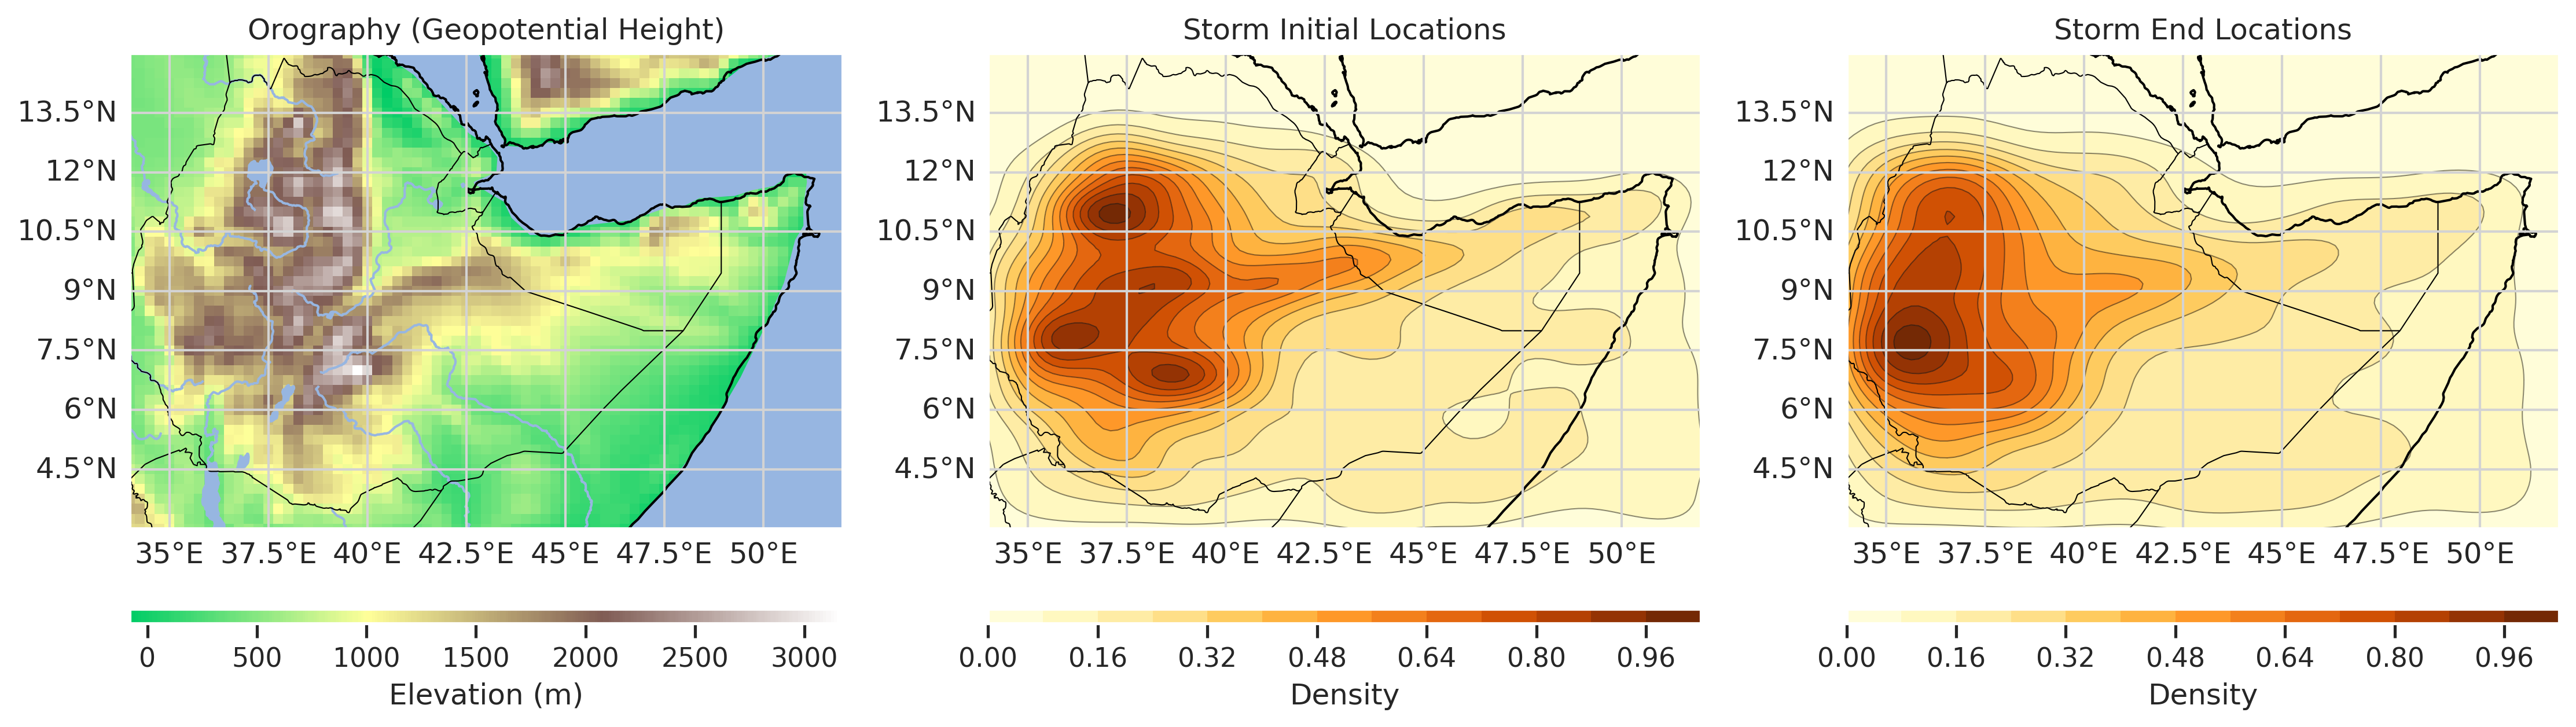
\includegraphics[width=\textwidth]{../figures/generated/orography_storm_init_end_kde.png}
    \caption{Storm First and Last Observation by Location.}
    \label{fig:orography_storm_init_end_kde}
\end{figure}

\begin{figure}[h]
    \centering
    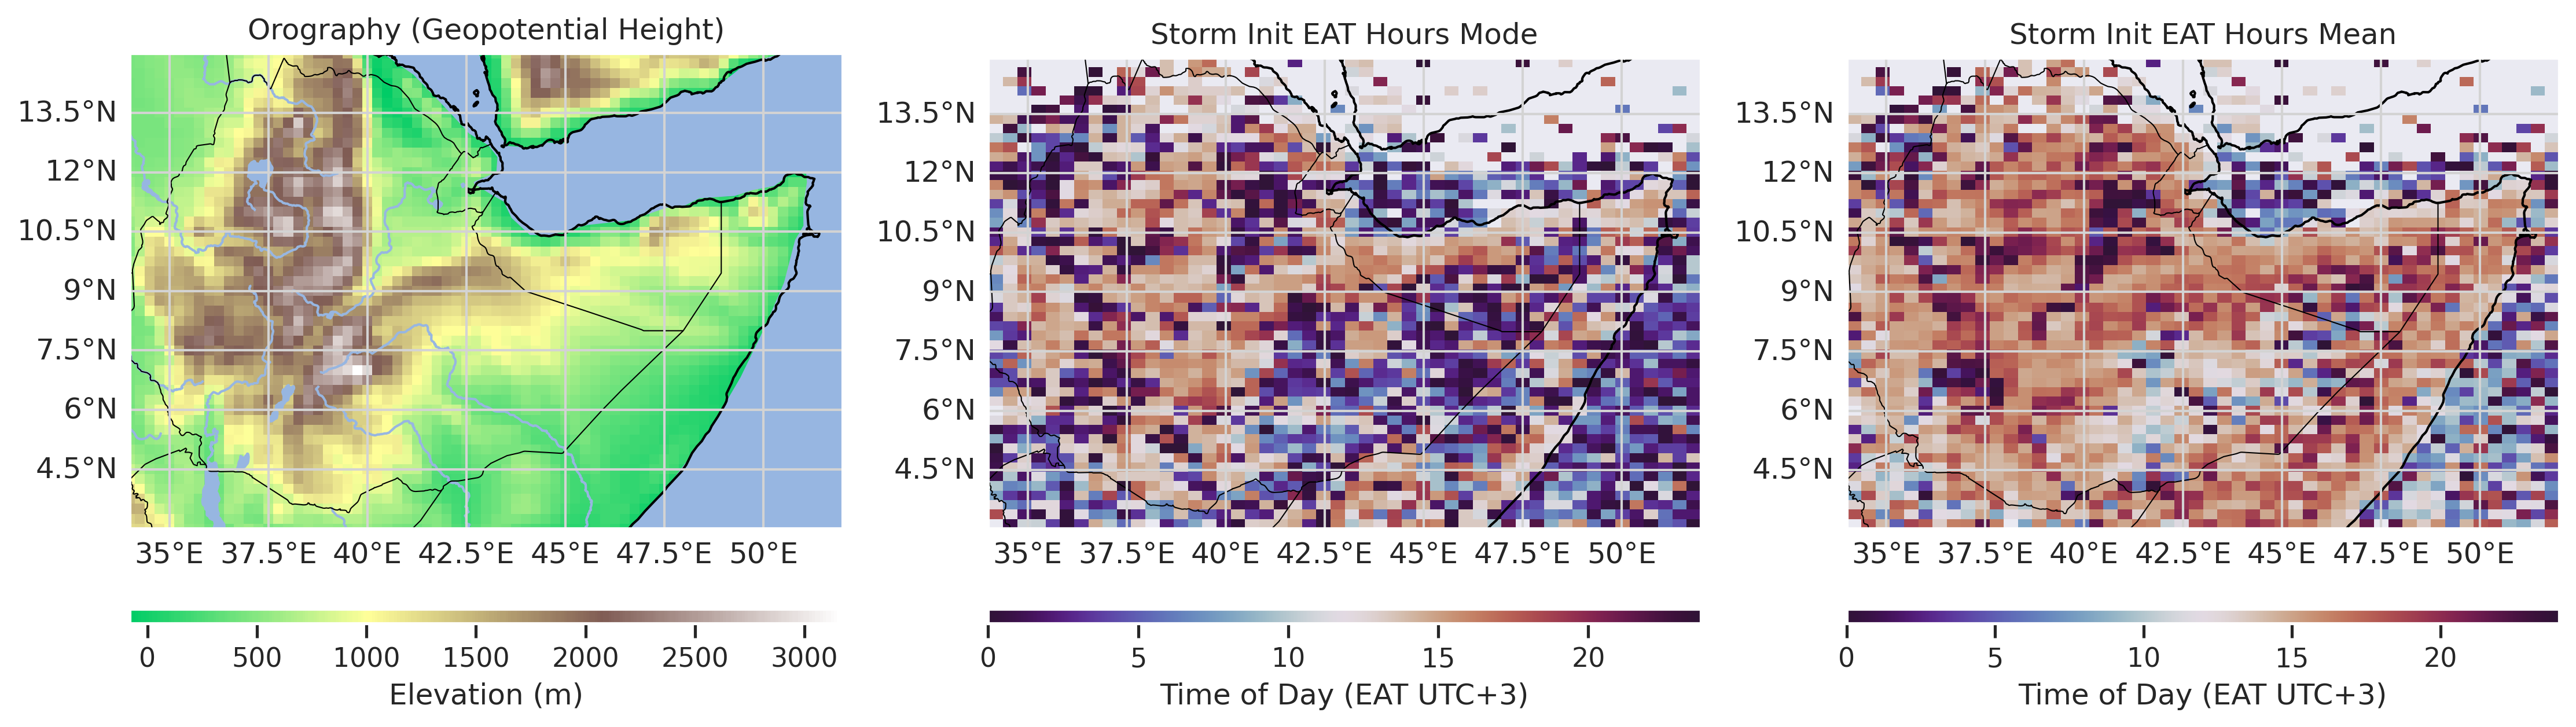
\includegraphics[width=\textwidth]{../figures/generated/orography_storm_init_eat_hours_mode_mean.png}
    \caption{Storm Genesis Local Time by Location.}
    \label{fig:orography_storm_init_eat_hours_mode_mean}
\end{figure}

\section{Experimental Setup}

For all experiments listed below, two models were trained on two different feature sets: all available features and only ERA5 meteorological features. This approach allows for a comparison of model performance when utilising a focused subset of variables. While it is clear from the manual exploration above that storm location and orography will play a major role, it is possible that those features could confound the effects of other environmental factors like soil moisture or skin temperature. Thus, through this setup, we ensure that one model is exclusively learning from the meteorological conditions. If model performance differs significantly, this would imply that the geographic, topological, or temporal features contain unique information not captured by the meteorological features. Through a comparison of relative feature importance of the meteorological features, we can also gain insights into their interaction with the other features. In addition, for the storm aggregate prediction tasks, two additional models were trained using only the first observation of each storm, again comparing all features versus only ERA5 features. This aspect of the setup aims to evaluate the predictive power of initial storm observations.

\section{Predict Storm Aggregate Features}

These experiments aim to predict the overall characteristics of a storm based on its initial observation.

\subsection{Storm Max Intensity}

\subsubsection{All Observations}

\begin{figure}[h]
    \centering
    \missingfigure{2x2 Subplots: Row 1: Actual vs Predicted scatter with regression, Row 2: SHAP beeswarm top features.}
    \caption{Comparison of performance and top features for storm max intensity.}
    \label{fig:storm_max_intensity_summary}
\end{figure}

\subsubsection{First Points Only}

\begin{figure}[h]
    \centering
    \missingfigure{2x2 Subplots: Row 1: Actual vs Predicted scatter with regression, Row 2: SHAP beeswarm top features.}
    \caption{Comparison of performance and top features for storm max intensity (First Points Only).}
    \label{fig:storm_max_intensity_first_points_summary}
\end{figure}

\subsection{Storm Direction}

\subsubsection{All Observations}

\begin{figure}[h]
    \centering
    \missingfigure{2x2 Subplots: Row 1: Actual vs Predicted scatter with regression, Row 2: SHAP beeswarm top features.}
    \caption{Comparison of performance and top features for storm direction.}
    \label{fig:storm_direction_summary}
\end{figure}

\subsubsection{First Points Only}

\begin{figure}[h]
    \centering
    \missingfigure{2x2 Subplots: Row 1: Actual vs Predicted scatter with regression, Row 2: SHAP beeswarm top features.}
    \caption{Comparison of performance and top features for storm direction (First Points Only).}
    \label{fig:storm_direction_first_points_summary}
\end{figure}

\section{Predict Immediate Characteristics at an Observation}

These experiments aim to predict the immediate characteristics of a storm based on its current observation.

\subsection{Intensification}

\begin{figure}[h]
    \centering
    \missingfigure{2x2 Subplots: Row 1: Actual vs Predicted scatter with regression, Row 2: SHAP beeswarm top features.}
    \caption{Comparison of performance and top features for intensification.}
    \label{fig:obs_intensification_summary}
\end{figure}

\subsection{Direction}

\begin{figure}[h]
    \centering
    \missingfigure{2x2 Subplots: Row 1: Actual vs Predicted scatter with regression, Row 2: SHAP beeswarm top features.}
    \caption{Comparison of performance and top features for direction.}
    \label{fig:obs_direction_summary}
\end{figure}

\subsection{Distance}

\begin{figure}[h]
    \centering
    \missingfigure{2x2 Subplots: Row 1: Actual vs Predicted scatter with regression, Row 2: SHAP beeswarm top features.}
    \caption{Comparison of performance and top features for distance.}
    \label{fig:obs_distance_summary}
\end{figure}

\subsection{Precipitation}

\begin{figure}[h]
    \centering
    \missingfigure{2x2 Subplots: Row 1: Actual vs Predicted scatter with regression, Row 2: SHAP beeswarm top features.}
    \caption{Comparison of performance and top features for precipitation.}
    \label{fig:obs_precipitation_summary}
\end{figure}
    \chapter{Discussion}
\label{ch:discuss}
\todo{in progress}

This chapter discusses the implications of the findings, the limitations of the study, and potential directions for future research.

\section{Model Performance and Predictability}

\subsection{First Points Only vs All Points}

Models trained on only the first observation in each storm consistently underperformed compared to those trained on all available observations. This suggests that incorporating the full temporal evolution of storms provides valuable information for prediction.

\subsection{Storm Direction and Distance}

As shown in Tables \ref{tab:storm_direction_results} and \ref{tab:obs_experiment_results} respectively, storm direction models perform well, but models predicting the next direction and distance of the storm at an observation perform poorly. This could be due to several factors. The calculation of the next direction relies on the centroid of the storm provided by \cite{Hill2023}. For \acrshortpl{mcs}, the centroid might be weakly defined as the storm structure does not often have a clear center of circulation compared to other systems like tropical cyclones. For example, squall lines are linear features and the centroid location outputted by the tracking algorithm may vary significantly between each time step based on the shape and orientation of the line. This would lead to particularly noisy data. To mitigate this, future work might investigate smoothing the centroid trajectory to reduce noise and improve the reliability of movement estimates. For direction specifically, using categorical representations of the compass bearing or transforming the degrees using sine and cosine functions, could address the challenges of modelling circular data. Categorical approaches would be more intuitive, but sine and cosine transformations would preserve granularity at the cost of increased complexity and the need for multiple outputs.

\section{Future Work}

\subsection{Dataset Expansion and Feature Engineering}

The \acrshort{mcs} database used in this study was limited to storms which spent their entire lifecycle within the study region. Expanding the storm database to include storms that pass through the region, rather than only those that originate and terminate within it, might provide a more comprehensive dataset for analysis. 

Additional features, such as equivalent potential temperature, could be incorporated to enhance model inputs.

The use of supplementary data sources, including satellite imagery and precipitation data as demonstrated in the original paper \citep{Hill2023}, may further improve predictive capabilities. While the universal availability of \acrshort{era5} data makes it a more practical choice for widespread application, region-specific data or higher resolution products could offer enhanced detail and accuracy in certain contexts even if they are less accessible or reduce viable data coverage. For example, this thesis considered the inclusion of precipitation data from the Global Precipitation Measurement (GPM) mission, but ultimately did not include it due to over 70\% of storm observations lacking corresponding GPM data. Future work could explore methods to effectively integrate such datasets.

\subsection{Model Improvements and Explainability}

\begin{itemize}
    \item Explore the use of alternative machine learning algorithms and architectures to improve predictive performance.
    \begin{itemize}
        \item Investigating anomalous individual predictions using decision plots or force plots to quantify edge cases for the models.
    \end{itemize}
    \item Conducting further analysis on the interpretability of model predictions, potentially through the use of more advanced explainability techniques.
    \begin{itemize}
        \item Investigating anomalous individual predictions using decision plots or force plots to quantify edge cases for the models.
    \end{itemize}
\end{itemize}
    \chapter{Conclusion}
\label{ch:con}

Globally, \acrfullpl{mcs} are defined as ensembles of thunderstorms organised in lines or clusters that typically produce severe weather over significant periods of time and large areas. They are a major contributor to intense rainfall \citep{Houze2004}, accounting for over 60\% of extreme rainfall events in Ethiopia and Somalia \citep{Hill2023}. Their devastating impact causes loss of life and displacement and can even impact neighbouring countries \citep{Mamo2019,Mekuria2022,Legese2020,Zaroug2014}. 

While these systems are significant in size, the convective processes that drive their intensification and propagation have historically not been directly simulated but rather parametrised in \acrfull{nwp} models \citep{Stevens2019,Yano2018,Keane2025}. Recent developments in convection-permitting models show promise in representing \acrshortpl{mcs} but forecasting inaccuracies remain prevalent \citep{Feng2025,Yano2018}. The under-representation of high-quality data in the continent of Africa further exacerbates the challenge of understanding and predicting \acrshortpl{mcs} within the region \citep{Dinku2019,Kinyondo2018,Meque2021}. Consequently, this thesis applied a reusable framework, adapted from \cite{Hunt2024}, for predicting their behaviour using \acrfull{xai} techniques. 

Prerequisite to the approach, a dataset was created to capture relevant meteorological, geographic, and temporal features along the 27,982 storm tracks within the Horn of Africa selected from \cite{Hill2023}. Multiple \acrfull{xgb} models were then trained to predict specific variables as proxies for storm intensification and propagation. The models were optimised using hyperparameter tuning and their performance compared between similar experiments with different feature sets to assess the impact of feature selection. Finally, \acrshort{xai} techniques, particularly \acrshort{shap}, were used to interrogate the models' predictions and identify the key factors influencing storm behaviour.

In experiments predicting the maximum intensity of a storm and the rate of intensification, the explainability analysis reveals that the \acrfull{ml} models learned from meteorological variables, notably \acrfull{cape}, \acrfull{tcwv}, wind shear, skin temperature, and soil moisture as expected from established literature \citep{Barton2021,Taylor2017,Li2023,Klein2020,Klein2021}. However, the feature values' influence on intensification was counter-intuitive and suggested possible spurious correlations with geography or biases within the dataset. 

Models trained to predict the overall direction of a storm were reasonably skilful, but those trained to predict direction and distance to the next observation were lacking. As such, no explainability analysis was conducted. Noisy data or suboptimal feature representation may have contributed to their poor performance. Using all available storm observations in model training also leads to better predictive capacity, rather than restricting the training dataset to only first points. This highlights the importance of \acrshort{mcs} evolution in overall quantification of storm characteristics.

The research conducted exemplifies the potential of \acrshort{xai} techniques in understanding and interpreting the dynamics of \acrshortpl{mcs} and poses it as an informative tool for the future development of forecast systems in data-sparse regions. The methodology is generalisable across different geographies and storm types, as evidenced by its successful application to both Indian Monsoon \acrlong{lps} by \cite{Hunt2024} and \acrshortpl{mcs} in East Africa in this thesis.

\section{Future Work}
\label{sec:future-work}

\subsection{Deepening of Explainability Analysis}

Due to the limited time available for this thesis, the explainability analysis conducted was far from exhaustive. The approach of identifying candidate features for further geographic and temporal analysis using their correlation with latitude, longitude, and time was a rough heuristic which may have missed more subtle relationships within feature contributions. Future work should aim to develop more sophisticated methods or more exhaustively examine all top features if time permits.

Furthermore, the analysis primarily focused on global feature importance and summary plots. Future work could delve deeper into local explanations to understand individual predictions better. Initial candidate samples could be easily identified via predictions with anomalous \acrshort{rmse}. Special attention should be paid to instances where similar samples exist that were correctly predicted. To facilitate investigation, the SHAP library provides various visualisation tools, such as force plots and decision plots, which can be utilised to visualise which features contribute to the erroneous output. Such an approach could help identify specific conditions or feature interactions that lead to model errors, thereby guiding targeted model improvements or possibly uncovering edge-case MCS behaviour.

\subsection{Dataset Expansion and Feature Engineering}

The \acrshort{mcs} database used in this study was limited to storms which spent their entire lifecycle within the study region. Expanding the storm database to also include storms tracks that pass through the region might provide a more comprehensive dataset for analysis, especially on the edges of the domain. The domain itself might also be expanded or contracted to reduce geographic correlations apparent with some of the meteorological features. For example, expansion of the dataset east to include more of the Indian Ocean or southwest to include the continuation of the Ethiopia Highlands into Kenya could improve the coverage of oceanic \acrshortpl{mcs} and reduce spatial biases with orography respectively. A reduction of the domain, perhaps to solely capture \acrshortpl{mcs} over the Ethiopian Highlands, could also help eliminate these correlations.

The dataset could also be expanded with additional features, such as equivalent potential temperature. As displayed in table \ref{tab:era5-file-patterns}, equivalent potential temperature data was available from the \acrshort{era5} data, but it was not included due to time constraints. Conversely, some features might be removed, particularly ones which contribute little to model performance, to reduce overall dimensionality and possibly improve model generalisation.

\subsection{Modelling Improvements}

Given this study focuses on post-hoc, model-agnostic explainability methods, future work could explore the integration of more complex \acrshort{ml} models, such as \acrfullpl{dnn}, to potentially improve predictive performance. While these models are not inherently interpretable, the methodology of applying of SHAP to explain their predictions would remain mostly unchanged when compared this thesis. Alternatively, more advanced, model-specific explainability techniques, such as layer-wise relevance propagation, or partially interpretable models, like attention-based \acrshortpl{dnn}, could be implemented.

    \bibliography{references}
    
    \begin{appendices}
        \chapter{An Appendix Chapter (Optional)}
\label{appn:A}
% Optional chapter
Some lengthy tables, codes, raw data, length proofs, etc. which are \textbf{very important but not essential part} of the project report goes into an Appendix. An appendix is something a reader would consult if he/she needs extra information and a more comprehensive understating of the report. Also, note that you should use one appendix for one idea.

An appendix is optional. If you feel you do not need to include an appendix in your report, avoid including it. Sometime including irrelevant and unnecessary materials in the Appendices may unreasonably increase the total number of pages in your report and distract the reader.


    \end{appendices}
    
\end{document}
